\chapter{Moduli stabilisation: the Dine--Seiberg problem and the cosmological moduli problem}
\label{ch:L3}
\lecturedate{Lecture of 12 November 2026}

This lecture completes the general picture drawn in the previous two. Many statements are still made without derivation, deliberately: the aim is an overall view of how string compactifications connect with the real world, and of what can go wrong, before the material is written down in equations, starting in the next lecture with D-branes. The lecture has three parts. The first explains why moduli stabilisation, introduced at the end of \cref{ch:L2}, is particularly hard in the heterotic string, and why type IIB is better placed. The second discusses, in a toy model with a single modulus, the general difficulty of stabilising the moduli with quantum corrections while keeping the effective theory under control, the \emph{Dine--Seiberg problem}, and the idea that resolves it. The third explains, with a simple cosmological estimate, why the moduli must be heavier than about $30\TeV$: the \emph{cosmological moduli problem}.

\section{Why moduli stabilisation is hard in the heterotic string}
\label{sec:L3-heterotic}

The moduli of \cref{sec:L2-moduli}, the Kähler moduli $T_i$, the complex-structure moduli $U_a$ and the axio-dilaton $S$, have a flat potential at tree level, which leads to fifth forces and to a complete lack of predictivity (\cref{sec:L2-moduli-problem}). Moduli stabilisation is the study of the quantum corrections that generate a potential for them, lift the flat directions and make them massive; the minimum of the potential then fixes, or \emph{stabilises}, the moduli at a point where predictions become possible.

In the heterotic string this programme is problematic, for three reasons. The first was met in \cref{sec:L2-alphaGUT}: by \cref{eq:L2-V25} the string coupling cannot be small, to suppress higher string loops, while the volume is large, to suppress higher-derivative corrections, so the effective theory is hard to trust. In type II theories one can have both; this was known from the beginning, but since type II theories seemed to give no non-abelian gauge bosons in four dimensions (\cref{sec:L2-spectra}), the advantage did not seem to matter.

\subsection{Background fluxes}

The second reason is that a major source of the potential for the moduli are \emph{background fluxes}, generalisations of electromagnetic fluxes. By Gauss's law, the flux of the electric field through a sphere surrounding a charge measures the charge, and similarly for the magnetic flux of a monopole; such fluxes carry energy. In four-dimensional Minkowski space a background electromagnetic field would pick a direction and break Lorentz invariance, but in the extra dimensions nothing forbids it: turning on fluxes there is like giving the field a vacuum expectation value in the extra dimensions, leaving the four-dimensional Lorentz symmetry untouched. The energy of a flux through a sphere depends on the size of the sphere, and if the sphere is in the extra dimensions its size is set by the size and shape of $Y_6$, i.e.\ by the moduli. A non-zero flux is therefore a source of energy that depends on the moduli: a potential for them.

The fluxes of string theory are those of the $p$-form fields of \cref{tab:L2-spectra}. The simplest is that of the Kalb--Ramond field $B_{MN}$, present in every closed superstring theory, whose field strength is the antisymmetrised derivative
\begin{equation}
  H_3 = \dd B_2 ,\qquad
  H_{MNP} = 3\,\partial_{[M}B_{NP]} = \partial_MB_{NP} + \partial_NB_{PM} + \partial_PB_{MN} ,
  \label{eq:L3-H3}
\end{equation}
with forms identified with their components as in the conventions. This generalises the electromagnetic field strength, $F_2 = \dd A_1$, i.e.\ $F_{\mu\nu} = \partial_\mu A_\nu - \partial_\nu A_\mu$.
The flux of $H_3$ goes not through a sphere but through a \emph{three-cycle} $\Sigma_3$, a three-dimensional submanifold of $Y_6$ without boundary, something like a three-sphere. In the vacuum considered so far the flux was zero; the idea is now to allow
\begin{equation}
  \int_{\Sigma_3}H_3 \neq 0 .
  \label{eq:L3-flux}
\end{equation}
The energy of such a flux depends on the volume of the three-cycle, and the volumes of three-cycles are controlled, for example, by the complex-structure moduli, which set the shape of the extra dimensions. Fluxes therefore generate a potential for the moduli, as needed.

The fluxes, however, are sources of energy in the extra dimensions, and energy curves spacetime: the fluxes \emph{backreact} on the Calabi--Yau. A mild possibility is \emph{warping}, in which the metric changes only by a conformal factor and the internal space stays conformally Calabi--Yau. In the heterotic string this is not what happens in general: the backreaction is so strong that the extra dimensions are no longer a Calabi--Yau manifold, and the chain of consequences is
\begin{equation*}
  \begin{gathered}
    \text{non-zero fluxes backreact on } Y_6\\[-0.3ex]
    \Downarrow\\[-0.3ex]
    \text{unknown moduli space}\\[-0.3ex]
    \Downarrow\\[-0.3ex]
    \text{loss of control of the effective theory.}
  \end{gathered}
\end{equation*}
Without control of the geometry one cannot even write down the tree-level effective theory. These manifolds are generalisations of Calabi--Yau manifolds that mathematicians are still trying to understand. Such compactifications are not wrong, but at present it is hard to compute with them. In type IIB (but not in type IIA) this problem is absent: fluxes can be turned on to stabilise moduli without destroying the Calabi--Yau background.

\subsection{The visible sector and the moduli in the same bulk}

The third reason is that in the heterotic string all the degrees of freedom, those of the Standard Model as well as the moduli, come from closed strings and live in the bulk of $Y_6$. In type IIB the moduli are again closed-string modes, but the Standard Model cannot be, since the closed-string spectrum has no non-abelian gauge bosons (\cref{sec:L2-vectors}); it comes instead from open strings on D-branes (\cref{sec:L2-spectra}). The two tasks, reproducing the Standard Model and stabilising the moduli, then concern two different kinds of strings, which decouple at leading order: one can solve each problem separately and then combine the solutions into a consistent whole. In the heterotic string both have to be solved at once, which is clearly harder. It is hard to address at the same time
\begin{enumerate}
  \item the construction of the Standard Model, with the correct gauge group, the chiral spectrum and the Yukawa couplings, and
  \item moduli stabilisation.
\end{enumerate}

The heterotic string remains an active field; the point here was how these problems arose historically. In type IIB the first problem is absent, the fluxes do not destroy the Calabi--Yau, and the two tasks of the third decouple. Before turning to type IIB compactifications, we discuss the problems of moduli stabilisation in general, from the point of view of the effective theory.

\section{What moduli stabilisation requires}
\label{sec:L3-requirements}

In general there are hundreds of moduli, and models with many of them are very hard to discuss. A very simplified toy model already shows the main issues. Let $\phi$ denote collectively all the moduli; for simplicity we mostly consider a single one. (In this chapter $\phi$ is a generic modulus, not the dilaton; see the conventions.) At tree level the potential vanishes,
\begin{equation}
  V_{\text{tree}}(\phi) = 0 .
  \label{eq:L3-Vtree}
\end{equation}
The quantum corrections must make it non-zero, $V(\phi^I)\neq0$, and develop a minimum $\langle\phi^I\rangle$ with no flat direction, as in \cref{eq:L2-stabilisation}, so that all the moduli are massive, $m^2_{\phi^I}>0$. The masses must also be large enough: above about a meV, \cref{eq:L2-bound}, to avoid fifth forces, and, by a much stronger bound derived in \cref{sec:L3-CMP},
\begin{equation}
  m_{\phi^I}\gtrsim30\TeV\qquad\text{for all } \phi^I ,
  \label{eq:L3-CMP-bound}
\end{equation}
to avoid the so-called \emph{cosmological moduli problem}.

The bound can be evaded or weakened in some models, but its origin is generic. Scalar fields with gravitational couplings easily come to dominate the energy density of the early universe: they behave as matter, so that between inflation and the late epochs of matter and cosmological-constant domination they produce an extra epoch dominated by the moduli. If stable, they overclose the universe; if they decay while dominating, the radiation they release dilutes everything produced before, and spoils Big Bang nucleosynthesis, whose predictions for the abundances of the light elements fit the data extremely well. Moduli heavier than about $30\TeV$ decay before nucleosynthesis starts, and are harmless for it. The argument is made quantitative in \cref{sec:L3-CMP}.

This is a very large mass for fields that are massless at tree level. It also has an interesting connection with supersymmetry: the effects that break supersymmetry generally also give mass to the moduli, and if the same mechanism gives mass to the squarks, the sleptons and the gauginos, the cosmological bound may indicate that the supersymmetric particles are heavy too, at least some $30$ to $100\TeV$.

Finally, the minimum must lie where the effective theory is under control. Since the strength of the couplings is itself set by the moduli, one proceeds as in \cref{sec:L1-scales}: assume weak coupling, keep only the leading quantum corrections, compute the potential they generate, and check a posteriori that its minimum is at weak coupling; if it is not, the result must be thrown away. The difficulty of meeting this condition is the \emph{Dine--Seiberg problem}~\cite{DineSeiberg}, made explicit by the toy model of \cref{sec:L3-dine-seiberg}. Part of the difficulty is that $V_{\text{quantum}}(\phi)$, unlike $V_{\text{tree}} = 0$, requires computations beyond tree level.

\section{Three kinds of quantum corrections}
\label{sec:L3-corrections}

In an effective theory derived from string theory the potential receives, beyond tree level, three types of quantum corrections:
\begin{equation}
  V_{\text{quantum}} = V_{g_s} + V_{\alpha'} + V_{\text{np}} .
  \label{eq:L3-Vquantum}
\end{equation}
The first are loop corrections, as in quantum field theory, controlled by the string coupling. The second are the higher-derivative $\alpha'$ corrections of \cref{sec:L1-control}, present already at tree level in $g_s$, which vanish in the point-particle limit $\alpha'\to0$. Both are perturbative: the first are loops in spacetime, the second loops in the worldsheet theory. The third are non-perturbative, both in $g_s$ and in $\alpha'$.

\emph{String loops.} The string-loop corrections scale as
\begin{equation}
  V_{g_s} = \sum_{m\ge1}g_s^m\,V_{(m)}(\text{moduli}) ,
  \label{eq:L3-Vgs}
\end{equation}
with $m$ the number of loops and coefficients $V_{(m)}$ that depend on the moduli. But $g_s$ is itself a modulus, $g_s = 1/\langle\mathrm{Re}\,S\rangle$ by \cref{eq:L2-ReS}: here the field $\phi$ of the toy model is $\mathrm{Re}\,S$, and to trust the expansion one needs
\begin{equation}
  g_s\ll1 \qquad\Longleftrightarrow\qquad \mathrm{Re}\,S\gg1 .
  \label{eq:L3-ReS}
\end{equation}
All the loops cannot be computed; in practice only the one-loop term can, and one works with it alone, assuming the higher ones to be small. The procedure is consistent if the resulting potential has a minimum at $\mathrm{Re}\,S\gg1$; if instead it just runs away in that region, two loops are needed as well, and so on.

In terms of $\phi = \mathrm{Re}\,S$, the loop expansion \cref{eq:L3-Vgs} becomes a series in powers of $1/\phi$,
\begin{equation}
  V_{g_s} = \frac{c_1}{\phi} + \frac{c_2}{\phi^2} + \frac{c_3}{\phi^3} + \dots ,
  \label{eq:L3-Vgs-phi}
\end{equation}
whose terms go like $g_s$, $g_s^2$, $g_s^3$, and so on, and the problem is immediately visible. The hard part is to compute the coefficients. If only $c_1$ is known, the potential $c_1/\phi$ has no minimum: it is a runaway. A minimum needs the second term as well, and if it comes from balancing the first term against the second, then at the minimum one loop and two loops are of the same size. For the minimum to be at $\phi\gg1$, $c_2$ must even be much bigger than $c_1$ in absolute value (and of opposite sign, for the two terms to balance). But if two loops are as big as one loop, why should three loops be negligible?

\emph{$\alpha'$ corrections.} The higher-derivative corrections have a similar structure,
\begin{equation}
  V_{\alpha'} = \sum_{m\ge2}\alpha'^m\,V_{(m)} ,
  \label{eq:L3-Valpha}
\end{equation}
but the sum now starts from $m = 2$, because supersymmetry makes the leading corrections vanish. Since $\alpha'$ is dimensionful, it must be compared with the size of the extra dimensions, and by \cref{eq:L1-invV}
\begin{equation}
  \alpha'\ll\mathrm{Vol}(Y_6)^{1/3} \qquad\Longleftrightarrow\qquad \Vol\gg1
  \label{eq:L3-largeV}
\end{equation}
parametrically: as in \cref{sec:L1-control}, the $\alpha'$ expansion is under control when the volume is large in string units.
The volume is a function of the Kähler moduli, so here the field $\phi$ of the toy model is $\Vol$: each power of $\alpha'$ comes with a power of $1/\Vol^{1/3}$, and $V_{\alpha'}$ is again an expansion in inverse powers of a modulus, like \cref{eq:L3-Vgs-phi}. The two expansions are intertwined: there is a whole $\alpha'$ expansion at tree level in $g_s$, another at one loop, and so on, and a generic correction is of a given order in both.

\emph{Non-perturbative corrections.} The last piece are corrections non-perturbative in $g_s$ or in $\alpha'$, the latter called \emph{worldsheet instantons}. Those non-perturbative in $g_s$ also form an expansion,
\begin{equation}
  V_{\text{np}} = \sum_{k\ge1}e^{-kA_k/g_s}\,V_{(k)} ,
  \label{eq:L3-Vnp}
\end{equation}
with positive constants $A_k$ and coefficients $V_{(k)}$ that can depend on the moduli. This expansion, too, can be trusted at small $g_s$, where the exponentials are very small. If moreover the $A_k$ are bigger than one, each further term carries an additional exponential suppression, $e^{-A/g_s}$, then $e^{-2A/g_s}$, and so on, and one can keep the leading term.

\section{The Dine--Seiberg problem}
\label{sec:L3-dine-seiberg}

To illustrate the Dine--Seiberg problem, consider the perturbative expansion alone, as one would naively do, since perturbative corrections are expected to dominate over non-perturbative ones, which are negligible if the constants $A_k$ in \cref{eq:L3-Vnp} are big. The potential then has the form
\begin{equation}
  V(\phi) = \frac{a}{\phi} - \frac{b}{\phi^2} + \frac{c}{\phi^3} + \mathcal O\Bigl(\frac{1}{\phi^4}\Bigr) ,
  \label{eq:L3-toy}
\end{equation}
where $\phi$ can be either $\mathrm{Re}\,S$ or the volume $\Vol$, both dimensionless, and the minus sign of the second term is written explicitly, so that the interesting case has $a,b,c>0$. One expects the three coefficients to be of order one,
\begin{equation}
  a\sim b\sim c\sim\mathcal O(1) ,
  \label{eq:L3-natural}
\end{equation}
as coefficients usually are. There are then two cases.

\emph{Trusting the effective theory: a runaway.} The effective theory can be trusted for $\phi\gg1$, a very big volume or a very small string coupling. But if all the coefficients are comparable, for $\phi\gg1$ the first term dominates,
\begin{equation}
  V(\phi)\simeq\frac{a}{\phi} ,
  \label{eq:L3-runaway}
\end{equation}
a runaway, shown in \cref{fig:L3-dine-seiberg}(a): the potential has no minimum, and the field is not stabilised. This need not be thrown away at once. At $\phi\gg1$, in a region of positive vacuum energy, the field could roll very slowly down a shallow, almost flat potential, and explain the present acceleration of the universe: this is the idea of \emph{quintessence}. But these corrections in general never give a potential flat enough for slow roll, and even if they did, the mass of the field would be of the order of the present Hubble scale, $H_0\sim10^{-33}\,$eV, and the field would mediate the fifth forces of \cref{sec:L2-moduli-problem}. So this does not really work.

\emph{Finding a minimum: tuning.} The other possibility is to use all the terms to find a minimum. Setting the first derivative to zero,
\begin{equation}
  V'(\phi) = -\frac{a}{\phi^2} + \frac{2b}{\phi^3} - \frac{3c}{\phi^4} = 0 ,
  \label{eq:L3-Vprime}
\end{equation}
gives a quadratic equation, $a\phi^2 - 2b\phi + 3c = 0$, with the two solutions
\begin{equation}
  \phi_{0,\pm} = \frac{b}{a}\Bigl(1\pm\sqrt{1-\frac{3ac}{b^2}}\Bigr) ,
  \label{eq:L3-roots}
\end{equation}
which are real for $b^2\ge3ac$. To check which is a minimum and which a maximum, one computes the second derivative,
\begin{equation}
  V''(\phi) = \frac{2a}{\phi^3} - \frac{6b}{\phi^4} + \frac{12c}{\phi^5} .
  \label{eq:L3-Vpp}
\end{equation}
At a critical point, eliminating $c$ with \cref{eq:L3-Vprime}, $V'' = 2(b-a\phi)/\phi^4$, and since $\phi_{0,-}<b/a<\phi_{0,+}$, for $b^2>3ac$
\begin{equation}
  V''(\phi_{0,-})>0\quad\text{(minimum)} ,\qquad
  V''(\phi_{0,+})<0\quad\text{(maximum)} .
  \label{eq:L3-minmax}
\end{equation}
To reproduce the cosmological constant, which today is almost zero, one also imposes that the potential vanish at $\phi_{0,-}$:
\begin{equation}
  V(\phi_{0,-}) = 0 \qquad\Longleftrightarrow\qquad ac = \frac{b^2}{4} .
  \label{eq:L3-minkowski}
\end{equation}
(Indeed, $V = V' = 0$ requires $a\phi^2 - b\phi + c = 0$ together with $a\phi^2 - 2b\phi + 3c = 0$, whose difference gives $\phi = 2c/b$, and substituting back gives $4ac = b^2$.) The potential then looks as in \cref{fig:L3-dine-seiberg}(b), and seems to reproduce the real world: the field is stabilised at the minimum, the vacuum energy there vanishes, and the potential is steep around it, so that the fluctuations have a large mass and can satisfy the bounds of \cref{sec:L3-requirements}.

\begin{figure}[tbp]
  \centering
  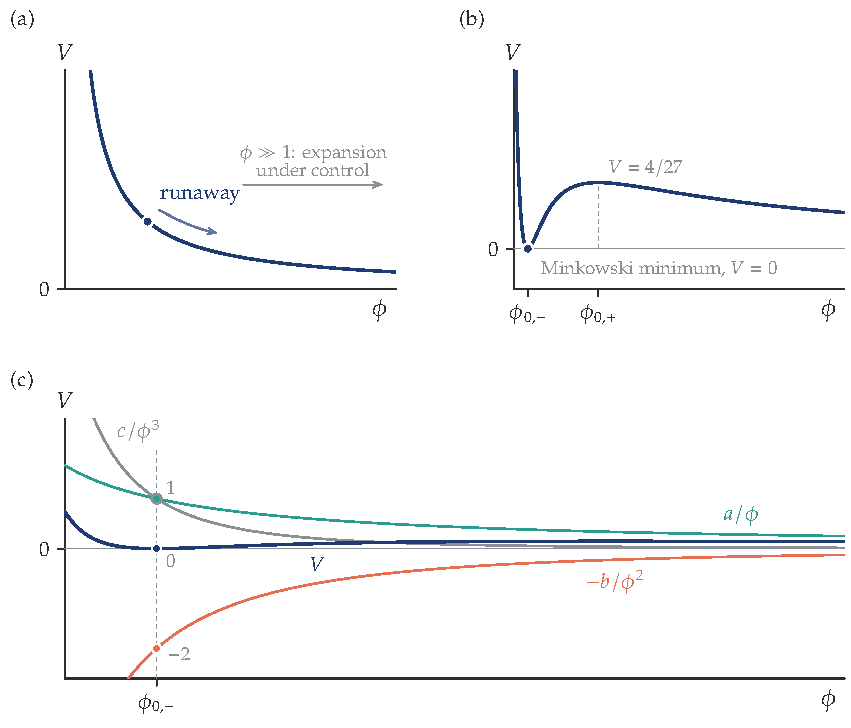
\includegraphics{fig_L3-dine-seiberg}
  \caption{The Dine--Seiberg problem in the toy model \cref{eq:L3-toy}. (a)~Where the expansion can be trusted, $\phi\gg1$, only the leading term survives, $V\simeq a/\phi$, and the modulus runs away to $\phi\to\infty$. (b)~Keeping three terms, with $ac = b^2/4$, gives a Minkowski minimum at $\phi_{0,-} = b/2a$ and a maximum at $\phi_{0,+} = 3b/2a$. (c)~At the minimum the three terms are of the same size, here $1$, $-2$ and $1$, and cancel.}\label{fig:L3-dine-seiberg}
\end{figure}

Can one then be in the limit $\phi\gg1$? With \cref{eq:L3-minkowski}, the expression \cref{eq:L3-roots} for the minimum becomes
\begin{equation}
  \phi_{0,-} = \frac{b}{2a}\gg1\qquad\text{if}\qquad b\gg a ,
  \qquad\text{and then}\qquad
  c = \frac{b^2}{4a}\gg b\gg a .
  \label{eq:L3-hierarchy}
\end{equation}
This contradicts \cref{eq:L3-natural}: one needs a hierarchy among the coefficients, $c\gg b\gg a$, which is a tuning. Is this natural? Is it even feasible? Moreover, the three contributions to the potential at the minimum are
\begin{equation}
  V(\phi_{0,-}) = \frac{a}{\phi_{0,-}} - \frac{b}{\phi_{0,-}^2} + \frac{c}{\phi_{0,-}^3}
  = \frac{2a^2}{b} - \frac{4a^2}{b} + \frac{2a^2}{b} = 0 .
  \label{eq:L3-terms}
\end{equation}
They cancel, but they are all of the same order, $a^2/b$. Why, then, should the term in $1/\phi^4$ be negligible? The only reason why one could still be at weak coupling, ignoring four loops, five loops and so on, is the tuning that makes $\phi$ big, $c\gg b\gg a$; but nothing guarantees that the same tuning does not also enhance the coefficient of $1/\phi^4$. Either one can trust the effective theory, and then there is no minimum, or one finds minima by balancing different terms of the same expansion, and then the result is always dirty. This is the \emph{Dine--Seiberg problem}, named after the paper that pointed it out~\cite{DineSeiberg}. It is not specific to the heterotic string, but a general problem of moduli stabilisation.

\subsection{The way out: balancing different expansions}
\label{sec:L3-way-out}

The Dine--Seiberg problem has been solved, by constructions found from the early 2000s onwards, which will be studied in equations towards the end of the course. The way out uses the fact that in string theory there is not just one expansion of the quantum corrections but three, the $g_s$, $\alpha'$ and non-perturbative expansions of \cref{eq:L3-Vquantum}. Each of them can be under control, with its first term much bigger than its second, and yet the first term of one expansion can balance the first term of another. A minimum found in this way can be fully under control. The idea is therefore to balance not different terms of the same expansion, but terms of different expansions: for example $\alpha'$ corrections against string-loop corrections, or perturbative against non-perturbative corrections. There are two famous solutions of this kind. One is \emph{KKLT}, from the initials of its authors, Kachru, Kallosh, Linde and Trivedi~\cite{KKLT}. The other, which appeared shortly afterwards, is the \emph{Large Volume Scenario} (LVS)~\cite{LVS}, in which, as the name says, the volume of the extra dimensions is very large.

\section{The cosmological moduli problem}
\label{sec:L3-CMP}

We now derive the bound \cref{eq:L3-CMP-bound}. There is no string theory in the argument, only the cosmology of a heavy scalar field with gravitational couplings, which must decay before Big Bang nucleosynthesis.

\subsection{A modulus displaced by inflation}

Suppose that the quantum corrections, in a scenario such as KKLT or the LVS, have produced a minimum in a regime in which the effective theory can be trusted, and shift the field so that the minimum is at zero. However complicated the potential is, around the minimum it is quadratic,
\begin{equation}
  V(\phi) = \frac12m_\phi^2\phi^2 \qquad\text{(at zero temperature)} ,
  \label{eq:L3-V0}
\end{equation}
where $\phi$ is now the canonically normalised modulus, of mass dimension one, and $m_\phi$ the mass of this spin-zero particle, which interacts gravitationally with everything.

In the very early universe, during inflation, the inflationary energy density, set by the Hubble rate as $\rho_{\text{inf}} = 3H^2\Mp^2$, contributes to the potential for the moduli, as any source of energy does, since the moduli couple gravitationally to it. A toy model of its effect is
\begin{equation}
  V(\phi) = \frac12m_\phi^2\phi^2 + \frac12H^2(\phi-\phi_0)^2
  \simeq \frac12H^2(\phi-\phi_0)^2 \qquad\text{for } H\gg m_\phi ,
  \label{eq:L3-Vinf}
\end{equation}
where the second term is the effect of inflation, with a coefficient of order one in general, here set to one. During inflation $H$ is much bigger than $m_\phi$: the inflationary Hubble scale can be as high as $10^{13}$--$10^{14}\GeV$ (present bounds on primordial gravitational waves require $H\lesssim5\times10^{13}\GeV$), while the modulus is much lighter. The minimum is then shifted to $\phi = H^2\phi_0/(H^2+m_\phi^2)\simeq\phi_0$, as in \cref{fig:L3-displacement}: in the early universe the field sits not at zero but at $\phi_0$. Since everything here is gravitational, the shift is expected to be of the order of the Planck scale, $\phi_0\sim\Mp$.

\begin{figure}[tbp]
  \centering
  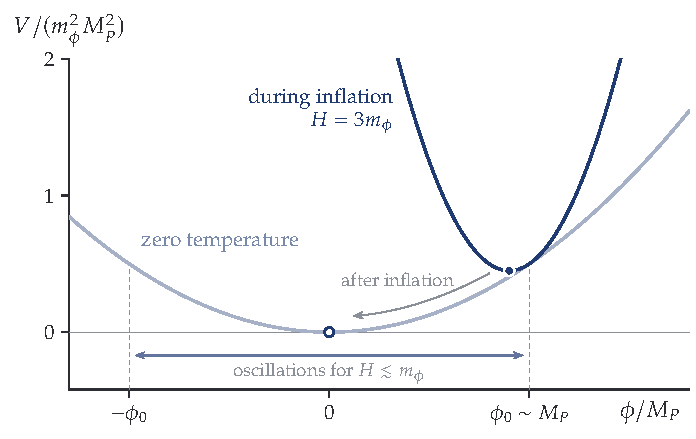
\includegraphics{fig_L3-displacement}
  \caption{A modulus during and after inflation. At zero temperature its potential is $\frac12m_\phi^2\phi^2$, with the minimum at $\phi = 0$ (light curve); during inflation the Hubble-induced term of \cref{eq:L3-Vinf}, with $H\gg m_\phi$ (here $H = 3m_\phi$), moves the minimum to $\phi\simeq\phi_0$ (dark curve). After inflation the field is left at $\phi_0$, far from the late-time minimum, and starts oscillating around it when $H\simeq m_\phi$.}\label{fig:L3-displacement}
\end{figure}

The evolution of the field is governed by the Klein--Gordon equation in an expanding universe, with the Friedmann--Lemaître--Robertson--Walker metric of the conventions. For a field that is homogeneous in space it reads
\begin{equation}
  \ddot\phi + 3H\dot\phi + m_\phi^2\phi = 0 .
  \label{eq:L3-KG}
\end{equation}
For $H = 0$ this is a harmonic oscillator. The term $3H\dot\phi$, due to the expansion of the universe, acts as friction, and for $H\gg m_\phi$ it dominates: the field is stuck at $\phi_0$, high up in the potential. As the universe expands, $H$ decreases, the potential approaches the zero-temperature one, \cref{eq:L3-V0}, and the friction becomes less and less important compared with the restoring force, until $H$ becomes of order $m_\phi$ and the field starts oscillating around the minimum:
\begin{equation}
  H_{\text{osc}}\simeq m_\phi .
  \label{eq:L3-Hosc}
\end{equation}
The initial amplitude is $\phi_0$, so the oscillations are large and the field stores energy instead of sitting at the minimum. While the field is stuck, its energy is only a small contribution to the vacuum energy; at the onset of the oscillations it is of the order of the potential,
\begin{equation}
  \rho_\phi^{\text{osc}}\simeq m_\phi^2\phi_0^2\simeq m_\phi^2\Mp^2 .
  \label{eq:L3-rho-phi}
\end{equation}

\subsection{Modulus domination and decay}

This energy density has to be compared with that of the standard cosmological history. After inflation the inflaton decays and reheats the universe: its energy goes into the particles of the Standard Model, which form a thermal bath and redshift as radiation. While the modulus is stuck it carries no energy density of its own, and all the energy is in radiation. But when $H$ drops to $m_\phi$, during radiation domination, part of the energy is in the oscillating $\phi$. The energy density of radiation at that time follows from the Friedmann equation, $3H^2\Mp^2 = \rho$:
\begin{equation}
  \rho_\gamma^{\text{osc}}\simeq H_{\text{osc}}^2\Mp^2\simeq m_\phi^2\Mp^2 .
  \label{eq:L3-rho-gamma}
\end{equation}
The two energy densities, \cref{eq:L3-rho-phi,eq:L3-rho-gamma}, are comparable: the modulus, which had no energy of its own, has as much energy as the whole Standard Model as soon as it starts oscillating.

As the universe expands both energy densities are diluted, but in different ways. A field oscillating coherently around its minimum is a condensate, a large number of quanta with zero momentum, and so it behaves as matter, which redshifts more slowly than radiation,
\begin{equation}
  \rho_\phi\propto a^{-3} ,\qquad \rho_\gamma\propto a^{-4} ,
  \label{eq:L3-redshift}
\end{equation}
where the scale factor $a$ grows with the expansion. Since the two start with comparable energies, $\phi$ very quickly comes to dominate the energy density of the universe.

This is the problem anticipated in \cref{sec:L3-requirements}. A stable modulus carries so much energy that it overcloses the universe, as too much dark matter. A modulus that decays into Standard Model particles converts all its energy into radiation, a huge injection of energy that dilutes all the particles present before, and with them the successful predictions for the abundances of the light elements. The decay happens when $H$ becomes of order the decay rate of $\phi$,
\begin{equation}
  H_{\text{dec}}\simeq\Gamma_{\phi\to\text{SM}} .
  \label{eq:L3-dec}
\end{equation}
since $1/H$ is the age of the universe and $1/\Gamma = \tau$ the lifetime of the particle. The history of the universe is then modified as in \cref{fig:L3-history}(a): after inflation and radiation domination comes an epoch of $\phi$ domination; when $\phi$ decays the universe returns to radiation domination, and then to matter and cosmological-constant domination as usual. Since everything produced before the decay is diluted, the decay must happen before Big Bang nucleosynthesis starts.

\begin{figure}[tbp]
  \centering
  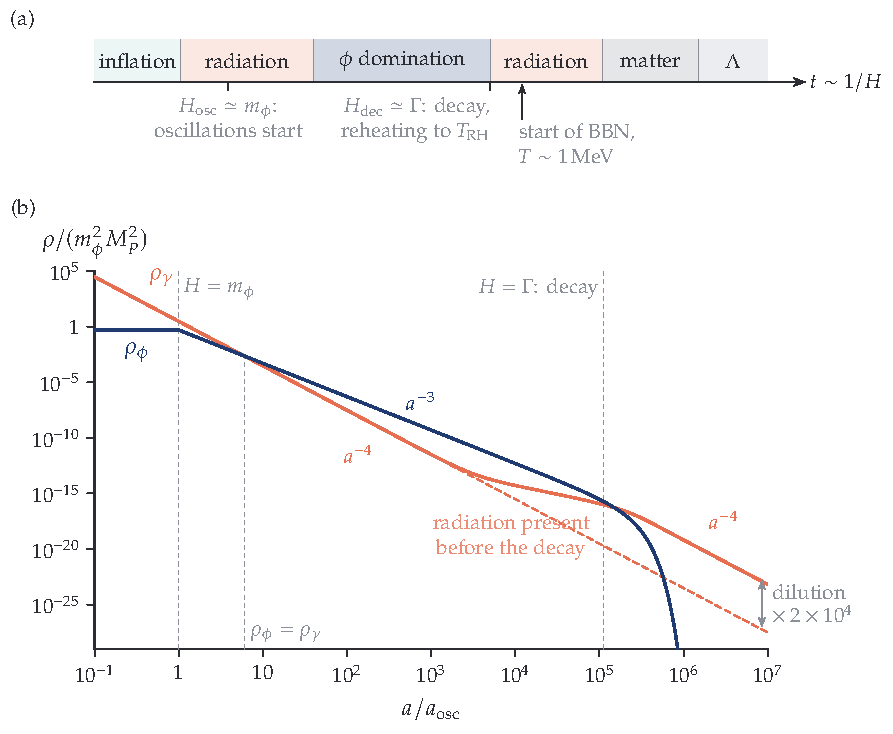
\includegraphics{fig_L3-history}
  \caption{Cosmological history with a displaced modulus. (a)~The sequence of epochs: inflation, radiation domination, domination by the oscillating modulus, radiation domination again after its decay, then matter and cosmological-constant domination. The modulus must decay before Big Bang nucleosynthesis starts. (b)~Energy densities of the modulus and of radiation as functions of the scale factor, from the onset of the oscillations at $H_{\text{osc}}\simeq m_\phi$ to the decay at $H_{\text{dec}}\simeq\Gamma$; the dashed line is the radiation present before the decay, diluted by it. The ratio $\Gamma/m_\phi = 10^{-8}$ is chosen for illustration; for a real modulus it is $(m_\phi/\Mp)^2\sim10^{-28}$.}\label{fig:L3-history}
\end{figure}

\subsection{The bound on the mass of the moduli}

To estimate $\Gamma_{\phi\to\text{SM}}$, note that the moduli couple to the gauge bosons: the gauge kinetic function, a function of the fields as seen in the supersymmetry course, depends in string compactifications on the moduli. Expanding it around the minimum gives a coupling of $\phi$ to two gauge bosons, suppressed by the Planck mass,
\begin{equation}
  \mathcal L_4\supset\frac{\phi}{\Mp}\,F_{\mu\nu}F^{\mu\nu} ,
  \label{eq:L3-phiFF}
\end{equation}
up to a coefficient of order one, through which the modulus decays as in \cref{fig:L3-decay}, very weakly. Dimensional analysis is enough to estimate the rate. It goes like the square of the coupling, $1/\Mp^2$, and has dimensions of a mass, so it must contain a mass cubed, and the only mass available in the decay into massless gauge bosons is $m_\phi$:
\begin{equation}
  \Gamma_{\phi\to\text{SM}}\simeq\frac{m_\phi^3}{\Mp^2} .
  \label{eq:L3-Gamma}
\end{equation}

\begin{figure}[tbp]
  \centering
  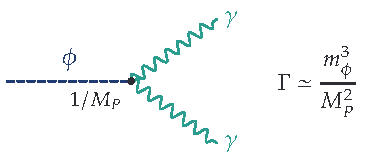
\includegraphics{fig_L3-decay}
  \caption{Decay of a modulus into two gauge bosons through the coupling \cref{eq:L3-phiFF}, with one vertex suppressed by $1/\Mp$, which gives $\Gamma\simeq m_\phi^3/\Mp^2$ (\cref{eq:L3-Gamma}).}\label{fig:L3-decay}
\end{figure}

The Hubble rate at the decay is then
\begin{equation}
  H_{\text{dec}}\simeq\Gamma_{\phi\to\text{SM}}\simeq m_\phi\Bigl(\frac{m_\phi}{\Mp}\Bigr)^2
  \simeq H_{\text{osc}}\Bigl(\frac{m_\phi}{\Mp}\Bigr)^2\ll H_{\text{osc}} ,
  \label{eq:L3-Hdec}
\end{equation}
by \cref{eq:L3-Hosc}, since the moduli are much lighter than the Planck scale: the moduli decay long after they start oscillating.

The decay reheats the universe, and $H_{\text{dec}}$ is the Hubble rate at the start of the new epoch of radiation domination, $H\simeq T^2/\Mp$ (see the conventions), at a temperature called the \emph{reheating temperature} $T_{\text{RH}}$. Hence
\begin{equation}
  H_{\text{dec}}\simeq\Gamma_{\phi\to\text{SM}}\simeq\frac{T_{\text{RH}}^2}{\Mp}
  \qquad\Longrightarrow\qquad
  T_{\text{RH}}\simeq\sqrt{\Gamma_{\phi\to\text{SM}}\Mp}\simeq m_\phi\sqrt{\frac{m_\phi}{\Mp}} ,
  \label{eq:L3-TRH}
\end{equation}
where the last step uses \cref{eq:L3-Gamma}.

For the decay to happen before Big Bang nucleosynthesis, the reheating temperature must exceed the temperature at which the light elements started to form, of order one MeV:
\begin{equation}
  T_{\text{RH}} > T_{\text{BBN}}\sim1\,\mathrm{MeV}\sim10^{-21}\Mp .
  \label{eq:L3-TBBN}
\end{equation}
With \cref{eq:L3-TRH} this gives $m_\phi^{3/2}\gtrsim10^{-21}\Mp^{3/2}$, i.e.
\begin{equation}
  m_\phi\gtrsim10^{-14}\Mp\sim10^4\GeV ,
  \label{eq:L3-mass-bound}
\end{equation}
a mass of order $10\TeV$. A more precise computation, keeping all the factors dropped in the signs $\simeq$, gives $30\TeV$: this is where the bound \cref{eq:L3-CMP-bound} comes from.

String compactifications must therefore make the moduli quite heavy. The bound can be evaded if the cosmological history has new features. The estimate assumed an initial displacement $\phi_0$ of order $\Mp$; if some mechanism made it much smaller, the energy stored in $\phi$ and the dilution would be much smaller too, and the cosmological history would have to be studied in detail. Alternatively, the displacement could be of order $\Mp$ but the moduli themselves diluted by something else in some epoch. So the bound \cref{eq:L3-CMP-bound} is much stronger than the bound \cref{eq:L2-bound} from fifth forces, and generically present, but it depends somewhat on the cosmology, whereas the much weaker one from fifth forces rests on observations made today.

In the next lecture we start looking at type IIB in equations: first D-branes and their effective action, then the bulk action, and how Calabi--Yau manifolds emerge.
